{\bf \em We propose here an optimized snapshot program to find the
first ever multiply-imaged supernova (SN).}  This program will exploit
a new HST capability enabled by the growing treasury of deep WFC3-IR
imaging on dozens of galaxy clusters that each contain many
multiply-imaged galaxies.  Along with the accompanying small GO
follow-up program (PI:Strolger), we will use this unprecedented
discovery to set the stage for the first ever use of a SN for time
delay cosmography -- a prospect initially conceived exactly fifty
years ago \citep{Refsdal:1964}.  Even with just a single SN time
delay, we will be able to measure \Ho\ to about 10\% precision {\em
without any reference to the local distance ladder}. This first SN
time delay will therefore deliver a valuable test of systematic
biases in other cosmological probes, and will serve as a pathfinder
for future large samples of lensed SN (e.g. from LSST).

\medskip
\noindent {\bf Motivation~~~} 
As light from a distant source passes through a galaxy cluster, strong
gravitational lensing causes multiple images to appear to the
observer.  The massive clusters in our target list all have dozens of
multiple images known, and it is from these multiply imaged galaxies
that we derive our primary constraints for cluster mass models
(REFERENCE??).  When a SN inevitably appears within one of these
multiply-imaged galaxies, it will of course be multiply-imaged itself.
Unlike the effectively static backgrond galaxies, a lensed SN is a
transient source, so we will observe the multiple images appear to us
separated by a time delay

\vspace{-5mm}
\hspace{-1.4cm}
\begin{tabular}{p{7cm}r}
% \dt = \frac{\Dl \Ds}{\Dls} ( 1 + z_l ) \phi
{\begin{align}
%\begin{equation}\label{eq:dt}
 %  \dt = \frac{\Dl \Ds}{\Dls} ( 1 + z_l ) \phi
%\end{equation}
  \dt = \frac{(1+z_L)}{c}\frac{\Dl \Ds}{\,\Dls} \phi, \label{eq:dt} \\
\mbox{where}~~ \phi = \frac{1}{2}(\theta-\beta)^2 - \psi(\theta), \label{eq:phi}
\end{align}}
&
\hspace{0.7cm}
\raisebox{-30mm}{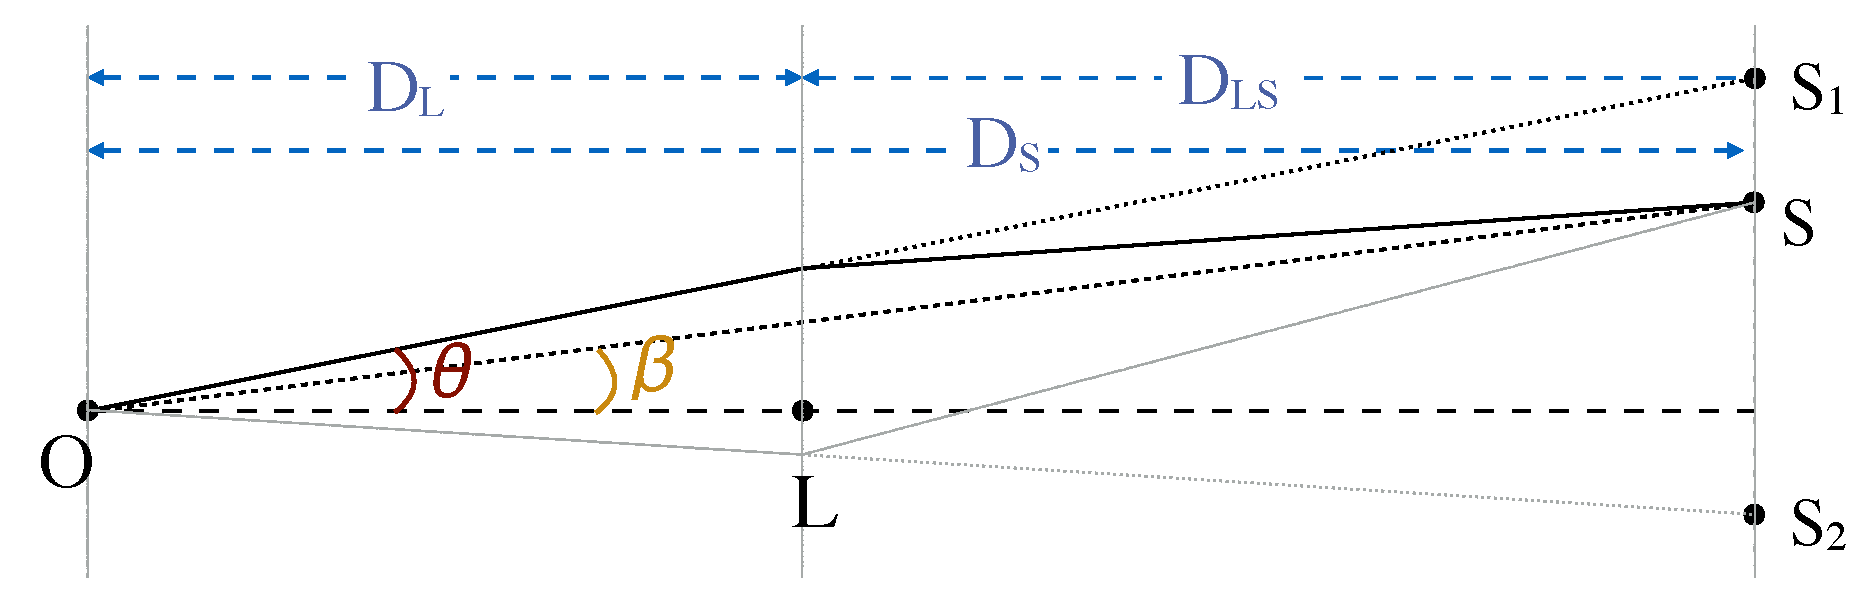
\includegraphics[width=0.52\textwidth]{FIG/lensingGeometry2}}
%\raisebox{-30mm}{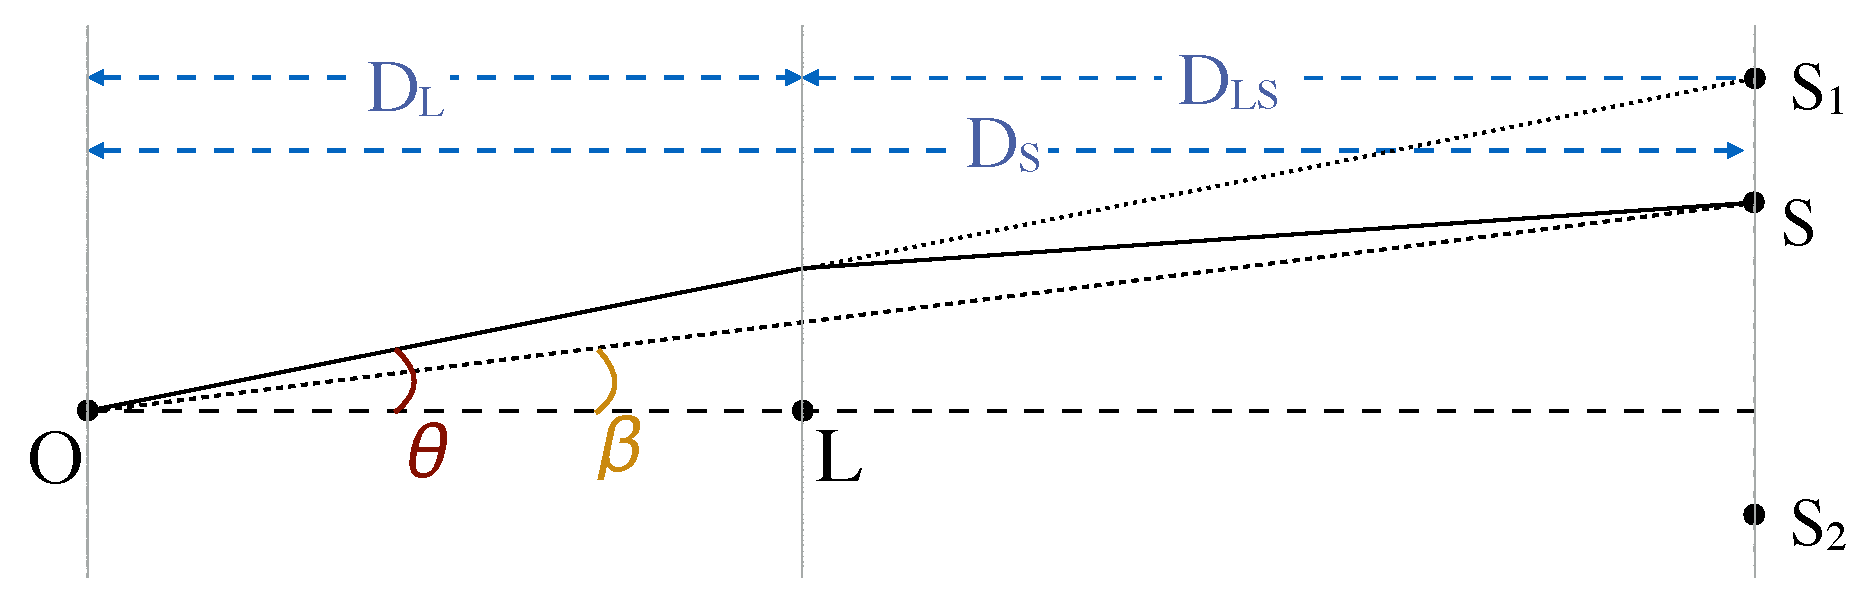
\includegraphics[width=0.5\textwidth]{FIG/lensingGeometry}}
\end{tabular}

\noindent and $z_L$ is the redshift of the lens, while \Dl, \Ds, 
and \Dls\ are angular diamater distances from the observer to the
lens, observer to source, and lens to source, respectively.  In
Eq.~\ref{eq:phi} for the time delay potential ($\phi$), the first term
gives the geometric delay due to light rays following different path
lengths to the observer, and the second term, $\psi$, is the
relativistic component due to differing values of the gravitational
potential along each path. The distance ratio $\Dl\Ds/\Dls$ in Eq. 1
carries a factor \Ho$^{-1}$, so if the lensing potential $\phi$ is
well known, this {\bf \em time delay cosmography provides a direct measurement of
the Hubble constant -- completely independent of the local distance
ladder.}

After several decades of dedicated effort and slow progress, this
field is now rapidly maturing \citep[see][for recent
reviews]{Jackson:2007,Treu:2010}.  The complete sample comprises
$\sim$20 time delay measurements, exclusively from {\em quasars}.
These are typically lensed by a single foreground galaxy, with only a
few magnified by galaxy clusters
\citep{Inada:2003,Inada:2006,Oguri:2008,Dahle:2013}.
As techniques for measuring the time delay \dt\ and modeling the
lensing potential $\psi$ have improved, there are now a few of these
lensed quasars that can jointly deliver an \Ho\ constraint with
$\sim$6\% precision \citep[e.g.][]{Suyu:2010,Suyu:2013}. The distances
derived from these time delay measurements are particularly
complementary to high-$z$ cosmological probes like the Cosmic
Microwave Background \citep[CMB; ][]{Linder:2011}.  Time delay
distances provide an especially powerful check for unknown
systematics, because -- unlike \SNIa -- each separate time delay
measurement can be individually quite precise and largely independent
of the rest of the sample \citep{Suyu:2013,Treu:2013}.  {\em A
measured time delay from even a single multiply-imaged SN would be a
valuable addition, and would provide a critical first step towards
future samples with over 100 SN time delays in the LSST era.}

A cluster-lensed SN would provide several distinct advantages that
make such an object particularly attractive for time delay
cosmography. First, the age of a SN relative to explosion can be
measured to within $\pm$3 days from light curve shape and color, or
from spectroscopic cross-correlation \citep{Filippenko:1997,
Blondin:2007}.  Thus the time delay measurement does not require
continuous long-term monitoring, as is needed for precise quasar time
delay measurements \citep[e.g.][]{Fohlmeister:2013, Tewes:2013a}.
Furthermore, with a cluster as the lensing object instead of a single
galaxy, there is a much lower likelihood of microlensing from
intervening compact objects (stars), and the microlensing effect can
be more easily disentangled from a SN light curve than from a
quasar \citep{Kolatt:1998,Tewes:2013b}.  Finally, if the lensed object
is a Type Ia SN (\SNIa), then the luminosity distance can be
independently constrained using light curve
fitting \citep{Phillips:1993}.  Some very recent work has even
suggested that it might also be possible to measure luminosity
distances from Type II-P SN light curves, though with lower
precision \citep{Anderson:2014, Sanders:2014}. With a known luminosity
distance, the source magnification can be directly measured, providing
powerful additional leverage for breaking degeneracies in the lens
model \citep{Kolatt:1998,Oguri:2003}.


% \bigskip
% 
% \textcolor{red}{SR: Maybe we need a separate (sub-)section that talks 
% about inverting the problem: using the SN magnification and time delay
% to test for systematics in the lens model instead of using the lens
% model as input for time delay cosmography.}  
% may also reveal systematics in the lens models themselves hidden
% otherwise (e.g. Oguri et al. **). 
% These systematics are a
% crucial factor in current Director's Discretionary Time studies of the
% high-redshift, magnified Universe such as the Frontier Fields program
% with HST${^1}$\footnotetext[1]{for which the co-PI A. Zitrin acted as
% an external lensing-science advisor, and in which we have (PI: Rodney)
% a program to search for general SNe}, for which the lens-magnification
% models are key.
% 
% \bigskip

\medskip
\noindent {\bf Predicted Yield~~~} 
To estimate the number of snapshots we need, we start with a
tabulation of the number of known multiply-imaged galaxies in the
fields of our target clusters (Table~\ref{tab:clusters} ** we need to
list the number of images, maybe not only the useful fraction?).  This
is a conservative approach, as it is quite possible to detect a
multiply-imaged SN even if the host galaxy is well below the current
detection thresholds for these cluster fields. The total yield of
strongly-lensed SN per snapshot is $N_{SN} = SNR_{M} \times
M_{gal} \times N_{gal} \times t_{vis}$.  Here $SNR_M$ is the SN rate
per unit mass, $M_{gal}$ is the average mass of a multiply-imaged
galaxy, $N_{gal}$ is the number of multiply imaged galaxies in the
field, and $t_{vis}$ is the length of time that any given SN is
visible to our snapshot survey.

Most of the lensed systems in our target list are at $z\sim 2$, in an
era near the peak of the cosmic star formation history, so we assume
that our average lensed galaxy is generating SN at a rate similar to
an Sc galaxy in our local universe: $SNR_{M} \sim0.2
(100 \mbox{yr})^{-1} (10^{10} \Msun)^{-1}$ for \SNIa\ and $0.7
(100 \mbox{yr})^{-1} (10^{10} \Msun)^{-1}$ for Type
II \citep{Mannucci:2005}.  We adopt an average stellar mass of
$M_{gal}=10^{10.7} \Msun$ \citep{Tomczak:2014}, and use the census of
multiply-imaged systems in Table~\ref{tab:clusters} to predict an
average of $N_{gal}\sim 35$ lensed galaxy images per
cluster$^{2}$.\footnotetext[2]{Note that we count each separate image of a
multiple-image set except the last one (one cannot measure a time delay
from the last appearance). The time delay between each image is of
order months or years, so each snapshot is essentially observing the
same galaxy at several widely-spaced epochs that can be treated as
independent.}  Using simulated SN light curves in 240 multiply-imaged
galaxies (Figure~\ref{fig:tvis}), we find an average $t_{vis}\sim 30$
days for \SNIa\ and $\sim$20 days for SN II.


With these relatively conservative estimates, we get $N_{SN}\sim
0.1$ SN per snapshot, including both Type Ia and II.  To give this
program a good chance at discovering a strongly lensed SN in Cycle 22,
we request 200 snapshots.  Assuming a realistic snapshot execution
rate of $\sim$30\%, this program should yield a sample of $\sim 6 \pm
4$ SN in one year.  Even if our yield prediction is biased high by a
factor of $\sim$2, we still have a better than 68\% chance to catch at
least one.  Given the intrinsic value of each lensed SN, even just a
single detection will nevertheless be an extraordinary step forward
for time delay cosmography.

Finally, we note that this snapshot program is designed mainly for
discovery. Follow-up observations will come from accompanying GO
program (PI: Strolger), using 12 orbits with ToO observations for immediate
confirmation of a SN candidate and measurement of the light curve.
Sometime in the future, a return campaign to catch the next image
would be needed to complete the time delay measurement, using HST,
ground-based AO systems, or possibly JWST, depending on the length of
the delay.


\begin{table}
\caption{Cluster Target List\label{tab:clusters}}
\begin{tabu}{llllcl}
\toprule
\toprule
Cluster & R.A. & Decl. & z & N$_{im}$ $^*$ & References \\
\midrule
\rowfont{\color{blue}}
Abell 2744\dag & 00:14:23.4 & -30:23:26 & 0.31 & 43  & Merten et al. 2011                                         \\
CL0024         & 00:26:35.0 & +17:09:43 & 0.39 & 20  & Zitrin et al. 2009a                                        \\
El Gordo       & 01:02:52.5 & -49:14:58 & 0.87 & 11  & Zitrin et al. 2013b                                        \\
\rowfont{\color{blue}}
Abell 370\dag  & 02:39:52.8 & -01:34:36 & 0.37 & 36  & Richard et al. 2009, ZFF                                   \\
Abell 383      & 02:48:03.4 & -03:31:44 & 0.19 & 18  & Zitrin et al. 2011b                                        \\
\rowfont{\color{blue}}
MACS0416\dag   & 04:16:08.4 & -24:04:21 & 0.40 & 36  & Zitrin et al. 2013                                         \\
MACS0647       & 06:47:50.3 & +70:14:55 & 0.58 & 20  & Zitrin et al. 2011, Coe et al. 2013                        \\
Bullet-a       & 06:58:37.9 & -55:57:00 & 0.3  & 10  & Bradac et al. **                                           \\
Bullet-b       & 06:58:37.9 & -55:57:00 & 0.3  & 11  & Bradac et al. **                                           \\
MACS0717-a     & 07:17:35.6 & +37:44:44 & 0.55 & 18  & Zitrin et al. 2009b, Limousin et al. 2012, Z14             \\
MACS0717-b     & 07:17:35.6 & +37:44:44 & 0.55 & 18  & Zitrin et al. 2009b, Limousin et al. 2012, Z14             \\
MACS0744       & 07:44:52.8 & +39:27:24 & 0.70 & 14  & Zitrin et al. 2011; 2014 in prep                           \\
Abell 611      & 08:00:56.8 & +36:03:23 & 0.21 & 12  & Newman et al. 2013, Z14                                    \\
\rowfont{\color{blue}}
MACS1149\dag   & 11:49:35.7 & +22:23:55 & 0.54 & 29  & Zitrin  \&  Broadhurst 2009, Zheng et al. 2012             \\
\rowfont{\color{blue}}
MACS1206\dag   & 12:06:12.1 & -08:48:04 & 0.44 & 33  & Ebeling et al. 2009, Zitrin et al. 2012                    \\
\rowfont{\color{blue}}
Abell 1689\dag & 13:11:34.2 & -01:21:56 & 0.19 & 117 & Broadhurst et al. 2005, Coe et al. 2010, Diego et al. 2014 \\
\rowfont{\color{blue}}
Abell 1703\dag & 13:15:03.7 & +51:49:27 & 0.28 & 36  & Limousin et al. 200*, Zitrin et al. 2010                   \\
RXJ1347        & 13:47:31.1 & -11:45:12 & 0.45 & 14  & K\"ohlinger \&  Schmidt 2014                               \\
MS1358         & 13:59:48.7 & +62:30:48 & 0.33 & 13  & Zitrin et al. 2011c                                        \\
Abell 1835     & 14:01:02.0 & +02:52:45 & 0.25 & 17  & Richard et al. 2010, Morandi et al. 2012                   \\
Abell 2218     & 16:35:54.0 & +66:13:00 & 0.18 & 18  & Kneib et al. 2004                                          \\
Abell 2261     & 17:22:27.2 & +32:07:57 & 0.22 & 18  & Coe et al. 2012                                            \\
MACS1931       & 19:31:49.6 & -26:34:32 & 0.35 & 10  & Z14                                                        \\
MACS2129       & 21:29:26.1 & -07:41:28 & 0.57 & 14  & Zitrin et al. 2011; Z14                                    \\
\rowfont{\color{blue}}
RXJ2248\dag    & 22:48:44.0 & -44:31:51 & 0.35 & 28  & Monna et al. 2013                                          \\
\bottomrule
% MACS0329   & 03:29:41.6 & -02:11:46 & 0.45 & 11 & Zitrin et al. 2012, Z14                       \\
% MACS0451   & 04:51:54.6 & +00:06:17 & 0.43 & 11                                                 \\
% MACS0454   & 04:54:11.1 & -03:00:53 & 0.54 & 11 & Zitrin et al. 2011                            \\
% CL1226     & 12:26:58.2 & +33:32:48 & 0.89 & 11 & Z14                                           \\
% MACS1423   & 14:23:48.3 & +24:04:47 & 0.54 & 11 & Limousin et al. 2010, Zitrin et al. 2011, Z14 \\
% MACS1720   & 17:20:16.8 & +35:36:26 & 0.39 & 11 & Z14                                           \\
% Abell 2390 & 21:53:55.8 & +17:43:34 & 0.23 & 7  & Frye et al. 1998                              \\
% MS2137     & 21:40:15.2 & -23:39:40 & 0.31 & 7  & Newman et al. 2013, Z14                       \\
% RXJ2129    & 21:29:40.0 & +00:05:21 & 0.23 & 9  & Richard et al. 2010, Z14                      \\
%\enddata
 \multicolumn{6}{p{\textwidth}}{* Approximate number of known strongly-lensed galaxy images
   within the WFC3-IR FOV, counting all instances of each lensed galaxy
   except the last (i.e. all independent lensed galaxy images that
   could deliver a SN time delay measurement).}\\
 \multicolumn{6}{p{\textwidth}}{ \textcolor{blue}{$\dagger$ Primary targets.} We will allocate more
   snapshots to these clusters that have especially strong lenses with
   many multiply-imaged galaxies and particularly good lens models.
   The unweighted average $N_{im}$ is $\sim$25, but we expect this
   weighted snapshot allocation to result in an actual mean of
   $N_{im}\sim 35$.}\\
%\tablenotetext{**}{ Key or latest references for the multiple image
%  compilation in each cluster. Z14 stands for ``Zitrin et al. 2014 in
%  prep" is a soon to be public paper describing our high-end mass
%  models already available online for the community, and multiple
%  images, for all 25 CLASH clusters. ``ZFF" refers to the internal
%  list of the Frontier Fields map making groups, for which Co-PI
%  Zitrin has contributed significantly for revising the multiple
%  images.}
\end{tabu}
\end{table}


%\insertfig{FIG/lightcurves.pdf}{ \label{fig:lightcurves} Lensed SN
%    light curves }

\insertfig{FIG/tvis_muz_20min.pdf}{\label{fig:tvis} 
Visibility time contours in the redshift-magnification plane. Using
simulated light curves of an average lensed Type Ia SN, we have
measured the expected visibility window (a.k.a the control time): the
number of days that the SN is above our detection threshold for a 20-minute
snapshot.  Solid lines plot contours of constant visibility time in
the $z-\mu$ plane at $t_{vis}=$100, 50, and 10 days.  Grey points mark
the measured magnifications and redshifts for 50 strongly-lensed
galaxy images from three of our primary cluster targets. }




